% !TEX program = xelatex
%Wzór dokumentu
%tu zmień marginesy i rozmiar czcionki
\documentclass[a4paper,12pt]{article}
\usepackage{inputenc}[utf8]
\usepackage[margin=2.8cm]{geometry}
\usepackage[polish]{babel}

%Lepiej tego nie zmieniaj, jak co to dodawaj pakiety
\usepackage{titlesec}
\usepackage{titling}
\usepackage{fancyhdr}
\usepackage{mdframed}
\usepackage{graphicx}
\usepackage{amsmath}
\usepackage{amsfonts}
\usepackage{multicol}
\usepackage{multirow}
\usepackage{listings}
\usepackage{caption}
\usepackage{float}
\usepackage{pdfpages}
\usepackage{tikz}
	\usetikzlibrary{arrows}
	\usetikzlibrary{patterns}
	\usetikzlibrary{decorations.pathmorphing}
\usepackage{pgf}
\usepackage[section]{placeins}



%inny wygląd
%\usepackage{tgbonum}


\usepackage{hyperref}
\hypersetup{
    colorlinks=true,
    linkcolor=blue,
    filecolor=magenta,      
    urlcolor=cyan,
}

\urlstyle{same}
%Zmienne, zmień je!
\graphicspath{ {./ilustracje/} }
\title{Tworzenie i uruchamianie prostych kontenerów w środowisku  docker-compose}
\author{Grzegorz Koperwas}
\date{\today}

%lokalizacja polska (odkomentuj jak piszesz po polsku)

\usepackage{polski}
\usepackage[polish]{babel} 
\usepackage{indentfirst}
\usepackage{icomma} 

\brokenpenalty=1000
\clubpenalty=1000
\widowpenalty=1000    

%nie odkometowuj wszystkiego, użyj mózgu
%\renewcommand\thechapter{\arabic{chapter}.}
\renewcommand\thesection{\arabic{section}.}
\renewcommand\thesubsection{\arabic{section}.\arabic{subsection}.}
\renewcommand\thesubsubsection{\arabic{subsubsection}.}

%Makra

\newcommand{\obrazek}[2]{
\begin{figure}[h]
    \centering
    \includegraphics[scale=#1]{#2}
\end{figure}
}     

\newcommand{\stopnie}{\ensuremath{^{\circ}}}

\newcommand{\twierdzonko}[1]{
    \begin{center}
    \begin{mdframed}
    #1
    \end{mdframed}          
    \end{center}
} 

\newcommand{\dwanajeden}[2]{
\ensuremath \left( \begin{array}{c}
    #1\\
    #2
\end{array} \right)
}  

%Stopka i head (sekcja której nie powinno się zmieniać)
\pagestyle{fancy}
\fancyhead{}
\fancyfoot{}

%Zmieniaj od tego miejsca
\rfoot{\thepage}
\lfoot{}
\lhead{}
\rhead{Ostatnia edycja: \today}
\renewcommand{\headrulewidth}{1pt}
\renewcommand{\footrulewidth}{1pt}



\begin{document}
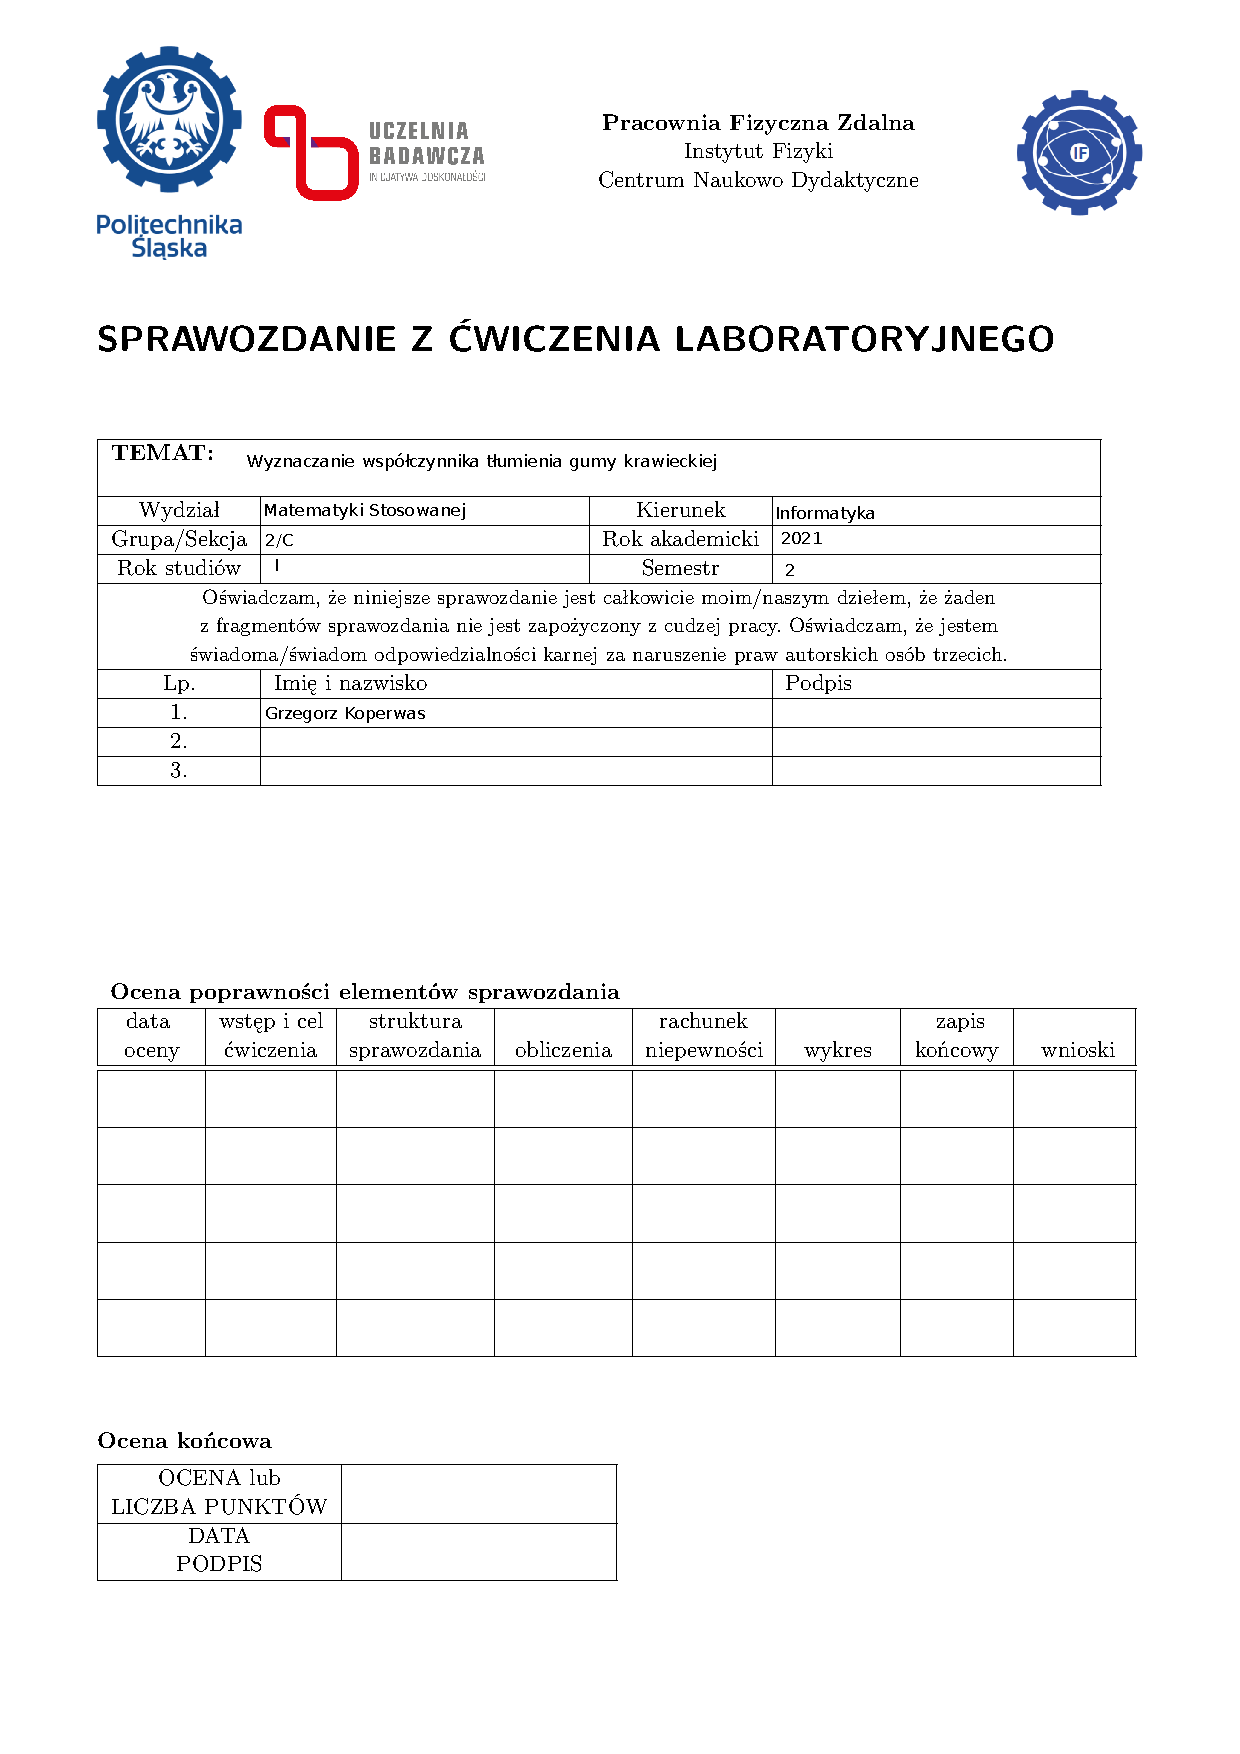
\includepdf[pages=-]{PFZ-StrTytulowa.pdf}

\section{Wstęp teoretyczny}

Celem doświadczenia było wyznaczenie współczynnika tłumienia gumki $\beta$ poprzez mierzenie przyspieszenia zawieszonej na niej masy.

\begin{figure}[h]
	\begin{tikzpicture}
		\fill [pattern = north east lines, draw=none, fill] (0, 0) rectangle (3, .3);
		\draw[thick] (0, 0) -- (3, 0);
		\node[rectangle, thick, inner sep=1.5mm, fill=black] (ball) at (1.5, -4) {\color{white}tel.};
		\draw[thin] (1.5, 0) -- (ball);
		\draw[->,thick] (ball) -- (1.5, -6) node[below] {$F_g$};
		\draw[->,thick] (ball) -- (1.5, -2) node[right] {$F_s$};
	\end{tikzpicture}
	\centering
	\begin{flushleft}
		Gdzie:
		\begin{itemize}
			\item \textbf{tel.} - zawieszona masa, w tym przypadku telefon z akcelerometrem.
			\item $F_g$ - siła ciążenia.
			\item $F_s$ - siła sprężystości.
		\end{itemize}
	\end{flushleft}
	\caption{Układ pomiarowy w stanie spoczynku}
\end{figure}

W eksperymencie mierzy się wartości maksymalne i minimalne przyspieszenia $a$, zatem do wyznaczenia współczynnika tłumienia możemy skorzystać logarytmicznego dekrementu tłumienia.


\begin{align}
	z_i & = \ln \frac{a\left(t_i\right)}{a\left(t_0\right)} \\
	T_i & = t_i - t_0
\end{align}\label{eq:ziti}

Gdzie $\beta$ to ujemne nachylenie wykresu stworzonego z par punktów $\left(T_i; z_i\right)$ dla kolejnych $t_i$ będących czasem w którym dokonano kolejnego pomiaru maksymalnego lub minimalnego przyspieszenia.

\clearpage

\section{Wyniki pomiarów:}

Tabela z czystymi wynikami pomiarów jest, ze względu na swój rozmiar, w załączonym Excelu.

Rozpatrywany jest przedział czasowy od $2,5s$ do $6,5s$.

\begin{figure}[h]
	\input{accel.pgf}%
	\centering
	\caption{Wycinek wykresu przyspieszenia od czasu}
\end{figure}

\subsection{Niepewności urządzeń pomiarowych}

Telefon, którym były dokonywane pomiary, posiada akcelerometr zintegrowany w układzie \texttt{BOSCH BMI120}.

W danych wygenerowanych przez użytą aplikację znajduje się informacja o rozdzielczości akcelerometru równej $0,0012 \frac{m}{s^2}$.

Według informacji producenta, w największym zakresie $S_{16g}$, czułość układu wynosi $\frac{1}{2048}g \approx 0,0048 \frac{m}{s^2}$ w temperaturze $25\stopnie C$. Odchylenie punktu zerowego wynosi zwykle $\pm 0,150g$ 

Na potrzeby pracy została przyjęta niepewność akcelerometru $u\left(a\right) = 0,0048 \frac{m}{s^2}$

\vspace{1cm}

Niepewność czasu jest nie została podana przez aplikację, zatem przyjmujemy $u\left(t\right) = 0,0010 s$. Pomiary były dokonywane co $0,0025s$.

\section{Przetwarzanie danych oraz obliczone wartości}

Z wykresu odczytujemy maksymalne oraz minimalne wartości:

\begin{table}[h]
	\begin{minipage}[c]{.45\textwidth}
		\begin{center}
			\begin{tabular}{ |c|c| }
				\hline
				t $\left[s\right]$ & $\left|a\right|$ $\left[\frac{m}{s^2}\right]$ \\\hline\hline
				3,135              & 3,460                                         \\\hline
				4,099              & 2,539                                         \\\hline
				4,808              & 1,777                                         \\\hline
				5,672              & 1,099                                         \\\hline
				6,396              & 0,733                                         \\\hline
			\end{tabular}
			\caption{Tablica dla wartości maksymalnych}\label{tab:max}
		\end{center}
	\end{minipage}\hspace{1cm}
	\begin{minipage}[c]{.45\textwidth}
		\begin{center}
			\begin{tabular}{ |c|c| }
				\hline
				t $\left[s\right]$ & $\left|a\right|$ $\left[\frac{m}{s^2}\right]$ \\\hline\hline
				2,717              & 3,506                                         \\\hline
				3,538              & 2,757                                         \\\hline
				4,422              & 2,196                                         \\\hline
				5,241              & 1,654                                         \\\hline
				6,025              & 1,152                                         \\\hline
			\end{tabular}
			\caption{Tablica dla wartości minimalnych}\label{tab:min}
		\end{center}
	\end{minipage}
\end{table}

Następnie dla każdego czasu $t_i$ w tabeli \ref{tab:max} oraz oddzielnie dla tabeli \ref{tab:min} obliczamy pary $z_i$ oraz $T_i$ zgodnie z równaniem (\ref{eq:ziti}).

\begin{figure}
	\input{lin.pgf}
	\centering
	\caption{Wykres dla obu zestawów wartości}
\end{figure}\label{rys:trends}

Dla prostych z wykresu na rysunku \ref{rys:trends} obliczamy współczynniki, gdzie wartość bezwzględna nachylenia $\left|m\right| = \beta$.

\vspace{5mm}

Zatem:

\vspace{3mm}

\begin{tabular}{lll}
	Dla maksimów:	& $\beta_{\max} = 0,485;$	& $u\left(\beta_{\max}\right) = 0,031$ \\
	Dla minimów:	& $\beta_{\min} = 0,328;$	& $u\left(\beta_{\min}\right) = 0,022$
\end{tabular}

\section{Wnioski}

Dla otrzymanych wcześniej wartości obliczamy średnią ważoną\footnote{Gdzie wagami są kwadraty odwrotności niepewności}, za niepewność przyjmujemy największą poprzednią wartość.

\vspace{5mm}

Ostatecznie:

\[
	\beta = 0,381;\: u\left(\beta\right) = 0,031
\]

\section{Sposoby na ograniczenie błędów}

Głównym problemem podczas przeprowadzania doświadczenia była mała amplituda drgań możliwa na zbyt krótkim kawałku gumki. Użycie dłuższej gumki pozwoliłoby na rejestrowanie drgań przez dłuższy okres.

Innym sposobem na ograniczenie błędów jest zwiększenie ilości dokonanych pomiarów. Zamiast rejestrować jedynie wartości minimalne i maksymalne z jednego pomiaru, lepiej było by dokonać dziesięciu (lub nawet 50) pomiarów. Częściowa automatyzacja\footnote{Został wykorzystany skrypt zwracający największą oraz najmniejszą wartość $a$ dla podanego $t$ z przedziału $\left( t - 0,1;\: t + 0,1 \right)$} procesu odczytywania wartości maksymalnego i minimalnego przyspieszenia została dokonana na potrzeby tego doświadczenia.

\end{document}
